\documentclass{article}

\usepackage{graphicx}
\usepackage{tikz}
\usepackage{tikzsymbols}
\usetikzlibrary{calc,patterns,shapes.geometric}
\pagestyle{empty}
\usepackage[margin=0pt]{geometry}
\geometry{papersize={14in,12in}}

\def\centerarc[#1](#2)(#3:#4:#5){\draw[#1] ($(#2)+({#5*cos(#3)},{#5*sin(#3)})$) arc (#3:#4:#5);}

\begin{document}
	\begin{figure}
		\centering
		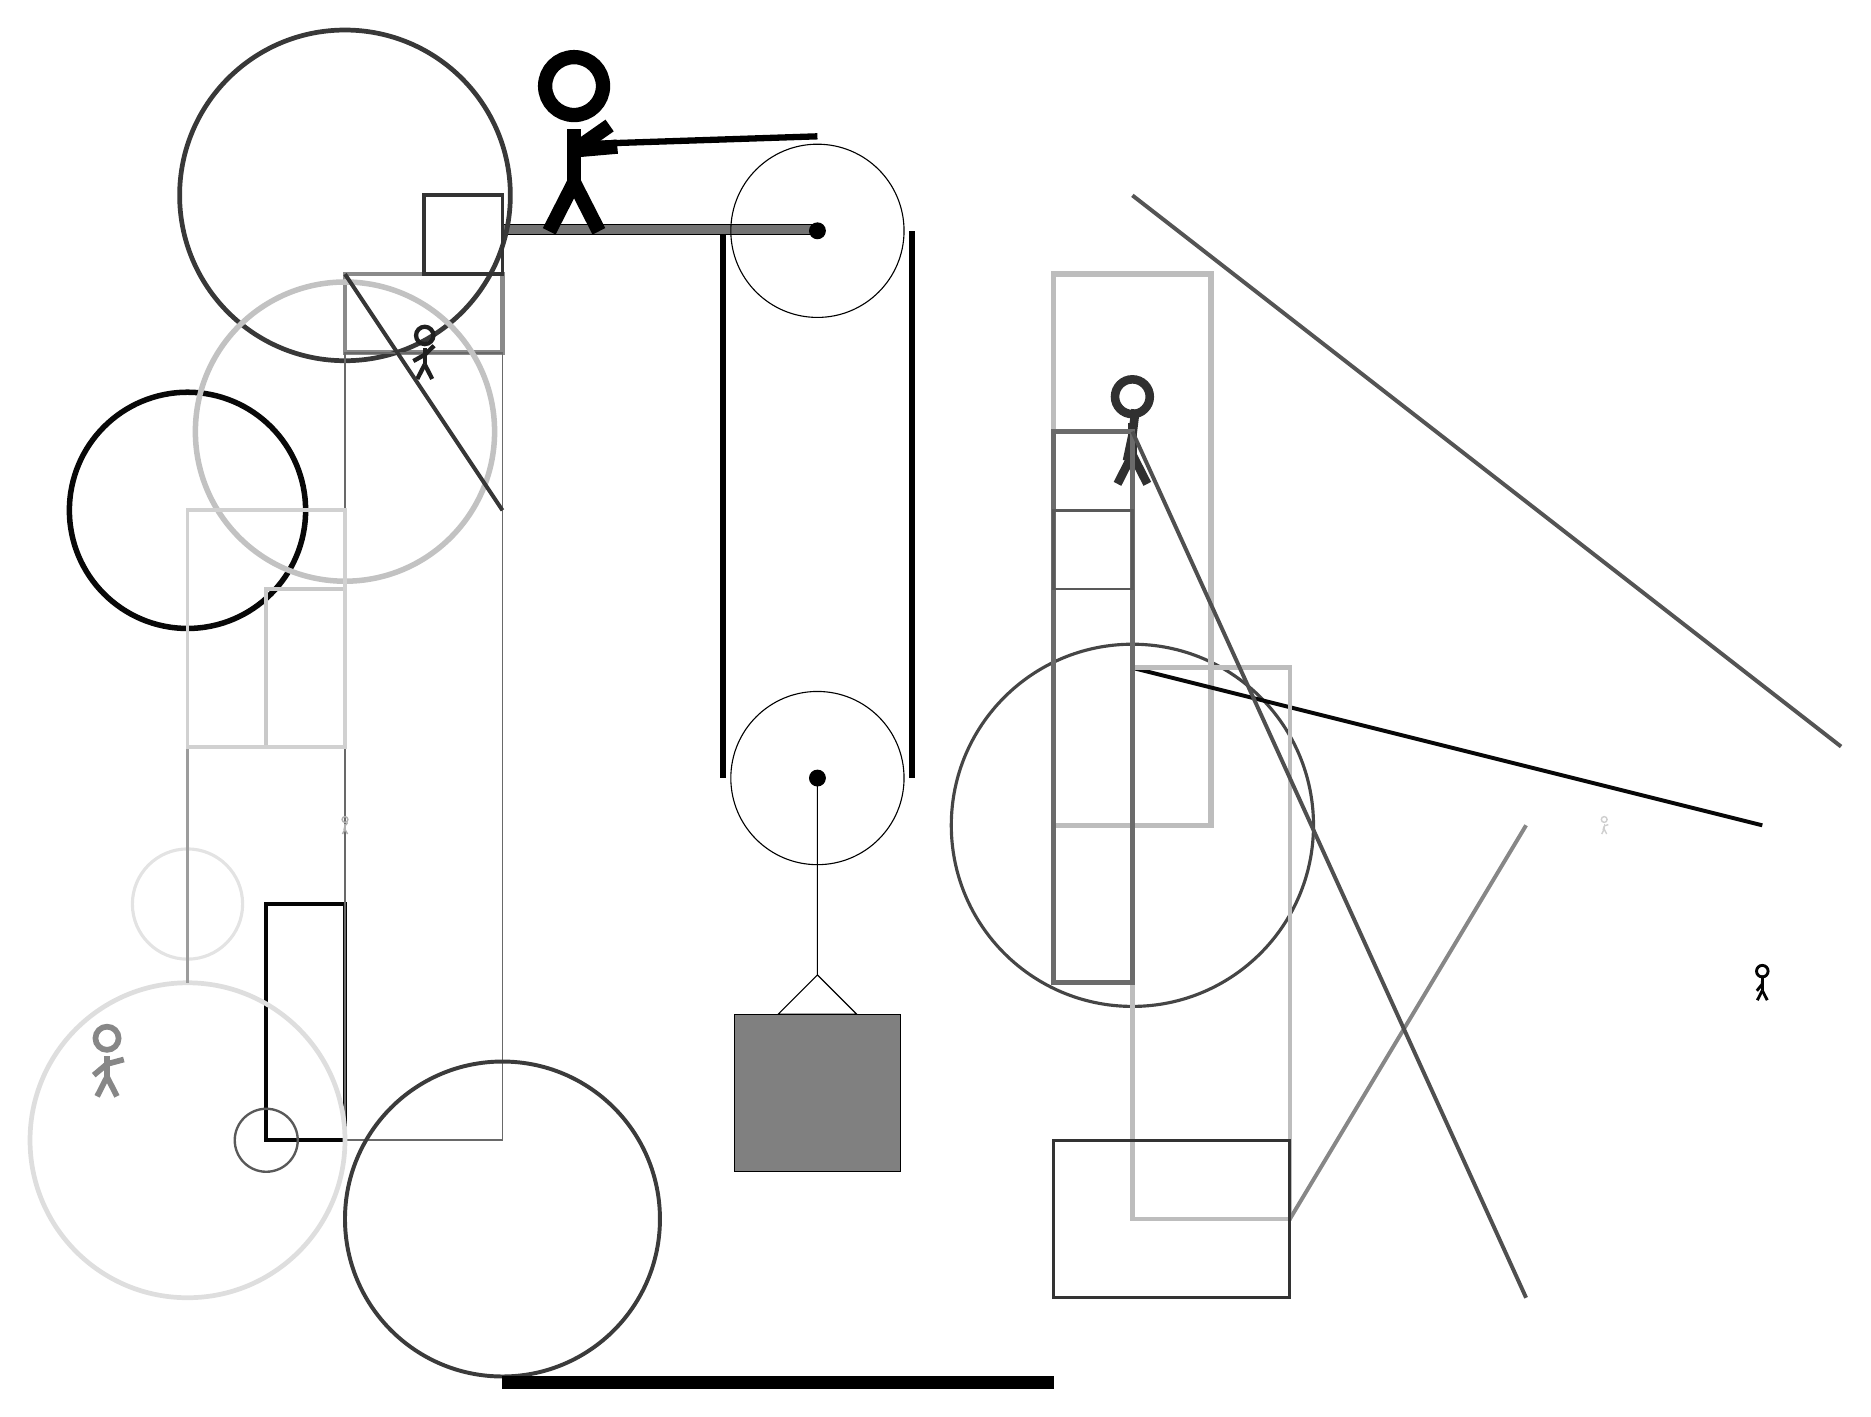
\begin{tikzpicture}
			%%%%% START %%%%%
			
			\draw[fill=black!55] (-2, 11.5) rectangle (2, 11.625);
			
			\draw[line width=0.6mm, color=black!46] (-2, 11) rectangle (-4, 10);
			
			\node[line width=0.2mm, color=black!81] at (6, 9) {\Strichmaxerl[6][78][83]};
			\node[line width=0.4mm, color=black!19] at (12, 4) {\Strichmaxerl[1][75][18]};
			\draw[line width=0.5mm, color=black!98] (-4, 3) rectangle (-5, 0);
			\draw [line width=0.6mm, color=black!78](-4, 12) circle (2.1);
			\draw [line width=0.4mm, color=black!73](6, 4) circle (2.3);
			\draw[line width=0.2mm, color=black!59] (-2, 0) rectangle (-4, 10);
			\node[line width=0.5mm, color=black!99] at (14, 2) {\Strichmaxerl[2][51][88]};
			\node[line width=0.6mm, color=black!88] at (-3, 10) {\Strichmaxerl[3][29][44]};
			
			\draw [line width=0.7mm, color=black!97](-6, 8) circle (1.5);
			\draw[line width=0.7mm, color=black!26] (7, 11) rectangle (5, 4);
			\draw[line width=0.5mm, color=black!97](6, 6) -- (14, 4);
			\draw[line width=0.6mm, color=black!26] (6, -1) rectangle (8, 6);
			
			\draw [line width=0.7mm, color=black!24](-4, 9) circle (1.9);
			\draw[line width=0.5mm, color=black!47](8, -1) -- (11, 4);
			\node[line width=0.4mm, color=black!47] at (-7, 1) {\Strichmaxerl[4][40][15]};
			
			\draw[line width=0.5mm, color=black!21] (-4, 5) rectangle (-5, 7);
			\draw [line width=0.4mm, color=black!11](-6, 3) circle (0.7);
			\draw [line width=0.5mm, color=black!77](-2, -1) circle (2.0);
			\draw[line width=0.4mm, color=black!80] (5, -2) rectangle (8, 0);
			\draw[line width=0.6mm, color=black!58] (6, 9) rectangle (5, 2);
			
			\draw[line width=0.5mm, color=black!79](-2, 8) -- (-4, 11);
			
			\draw [line width=0.3mm, color=black!65](-5, 0) circle (0.4);
			\draw[line width=0.5mm, color=black!67](6, 12) -- (15, 5);
			\draw[line width=0.5mm, color=black!80] (-3, 11) rectangle (-2, 12);
			
			\draw[line width=0.5mm, color=black!69](6, 9) -- (11, -2);
			\draw [line width=0.6mm, color=black!13](-6, 0) circle (2.0);
			\draw[line width=0.3mm, color=black!65] (5, 7) rectangle (6, 8);
			\node[line width=0.3mm, color=black!31] at (-4, 4) {\Strichmaxerl[1][76][52]};
			
			\draw[line width=0.5mm, color=black!39](-6, 2) -- (-6, 7);
			\draw[line width=0.5mm, color=black!18] (-4, 8) rectangle (-6, 5);
			
			
			\draw (2, 4.6) circle (1.1);
			\draw[fill=black] (2, 4.6) circle (0.1);
			
			\draw (2, 11.55) circle (1.1);
			\draw[fill=black] (2, 11.55) circle (0.1);
			
			\draw (2, 4.6) -- (2, 2.1) -- (1.5, 1.6) -- (2.5, 1.6) -- (2, 2.1);
			\draw[fill=black!50] (0.95, 1.6) rectangle (3.05, -0.4);
			
			\draw[line width=0.8mm] (0.8, 11.5) -- (0.8, 4.6);
			\centerarc[line width=0.8mm](2, 4.6)(180:360:1.2000000000000002);
			\draw[line width=0.8mm](3.2, 4.6) -- (3.2, 11.55);
			\centerarc[line width=0.8mm](2, 11.55)(0:90:1.2000000000000002);
			\draw[line width=0.8mm](2, 12.75) -- (-1, 12.65);
			
			\node at (-1, 12.65) {\Strichmaxerl[10][-175][35]};
			
			\draw[fill=black] (-2, -3) rectangle (5, -3.15);
			
			%%%%% END %%%%%
		\end{tikzpicture}
	\end{figure}	
\end{document}